\documentclass[12pt]{beamer}

\usetheme[white,sections]{Wisconsin}
\usepackage{fancyvrb}
\usepackage{color}
\usepackage[normalem]{ulem}
\usepackage{xcolor}
\usepackage{anyfontsize}
\usepackage{wrapfig}
\usepackage{graphicx}
\usepackage{tikz}
\usetikzlibrary{shapes.arrows}
\tikzset{
    myarrow/.style={
        draw,
        fill=orange,
        single arrow,
        minimum height=2.5ex,
        single arrow head extend=0.5ex
    }
}
\tikzset{
    mydoublearrow/.style={
        draw,
        fill=orange,
        double arrow,
        minimum height=10.5ex,
        single arrow head extend=1ex
    }
}

\newcommand{\arrowup}{%
\tikz [baseline=-0.5ex]{\node [myarrow,rotate=90] {};}
}
\newcommand{\arrowdown}{%
\tikz [baseline=-1ex]{\node [myarrow,rotate=-90] {};}
}
\newcommand{\doublearrow}{%
\tikz [baseline=-1ex]{\node [mydoublearrow,rotate=0] {};}
}


\begin{document}
\newcommand*{\alphabet}{ABCDEFGHIJKLMNOPQRSTUVWXYZabcdefghijklmnopqrstuvwxyz}
\newlength{\highlightheight}
\newlength{\highlightdepth}
\newlength{\highlightmargin}
\setlength{\highlightmargin}{2pt}
\settoheight{\highlightheight}{\alphabet}
\settodepth{\highlightdepth}{\alphabet}
\addtolength{\highlightheight}{\highlightmargin}
\addtolength{\highlightdepth}{\highlightmargin}
\addtolength{\highlightheight}{\highlightdepth}
\setbeamertemplate{bibliography entry title}{}
\setbeamertemplate{bibliography entry location}{}
\setbeamertemplate{bibliography entry note}{}
\newcommand*{\Highlight}{\rlap{\textcolor{HighlightBackground}{\rule[-\highlightdepth]{\linewidth}{\highlightheight}}}}
\setbeamertemplate{bibliography item}[text]
\setbeamercolor{section in toc}{fg=white}
\setbeamercolor{bibliography entry author}{fg=black}
\setbeamercolor{bibliography item}{fg=black}
\setbeamercolor*{bibliography entry title}{fg=black}
%\setbeamerfont{section number projected}{size=\tiny}
\setbeamerfont{section number projected}{size=\fontsize{6}{6}\selectfont}
\setbeamercolor{section number projected}{bg=UWRed,fg=white}
\hypersetup{linkcolor=white,urlcolor=white}

\AtBeginSection{\frame{\sectionpage}}
\defbeamertemplate{section page}{mine}[1][]{%
  \begin{centering}
    {\usebeamerfont{section name}\usebeamercolor[fg]{section name}#1}
    \vskip1em\par
    \begin{beamercolorbox}[sep=12pt,center]{part title}
      \usebeamerfont{section title}\insertsection\par
    \end{beamercolorbox}
  \end{centering}
}
\setbeamertemplate{section page}[mine]

%%%%%%%%%%%%%%%%%%%%%%%%%%%%%%%%%%%%%%%%%%%%%%%%%%%%%%%%%%%%%%%%%%%%%%%%%%%%%%%%
\title{Quality Assurance within the PyNE Open Source Toolkit}   
\author{Elliott Biondo$^1$, Anthony Scopatz$^1$, Matthew Gidden$^1$, \\ 
        Rachel Slaybaugh$^2$, Cameron Bates$^2$, Paul P.H. Wilson$^1$}
\institute{$^1$University of Wisconsin - Madison \\ 
           $^2$University of California, Berkeley}
\date{Nov. 11, 2014}
\frame[plain]{\titlepage \addtocounter{framenumber}{-1}} 

%%%%%%%%%%%%%%%%%%%%%%%%%%%%%%%%%%%%%%%%%%%%%%%%%%%%%%%%%%%%%%%%%%%%%%%%%%%%%%%%
%%%%%%%%%%%%%%%%%%%%%%%%%%%%%%%%%%%%%%%%%%%%%%%%%%%%%%%%%%%%%%%%%%%%%%%%%%%%%%%%
%%%%%%%%%%%%%%%%%%%%%%%%%%%%%%%%%%%%%%%%%%%%%%%%%%%%%%%%%%%%%%%%%%%%%%%%%%%%%%%%
\section{Introduction}
%%%%%%%%%%%%%%%%%%%%%%%%%%%%%%%%%%%%%%%%%%%%%%%%%%%%%%%%%%%%%%%%%%%%%%%%%%%%%%%%
%%%%%%%%%%%%%%%%%%%%%%%%%%%%%%%%%%%%%%%%%%%%%%%%%%%%%%%%%%%%%%%%%%%%%%%%%%%%%%%%
%%%%%%%%%%%%%%%%%%%%%%%%%%%%%%%%%%%%%%%%%%%%%%%%%%%%%%%%%%%%%%%%%%%%%%%%%%%%%%%%
\begin{frame}[fragile]
\frametitle{The PyNE toolkit}

\centerline{\bf Python for Nuclear Engineering:}
A trans-institutional, open source project for nuclear science and engineering analysis and simulations.

\centerline{
\includegraphics[width=2cm]{figures/pyne_icon_small.png}}

\begin{itemize}
\item{A library of tools, designed to be components of larger applications.}
\item{All code has a common Python interface}
\begin{itemize}
\item{A majority of code is written in C++ and wrapped with Python.}
\item{At one time: On GitHub.com's Top 25 ``trending'' C++ projects.}
\item{27 contributors}
\item{21 contributors with over 1000 lines of code/tests/documentation}
\end{itemize}
\end{itemize}


\end{frame}
%%%%%%%%%%%%%%%%%%%%%%%%%%%%%%%%%%%%%%%%%%%%%%%%%%%%%%%%%%%%%%%%%%%%%%%%%%%%%%%%
\begin{frame}[fragile]
\frametitle{The PyNE toolkit}

\begin{columns}
\begin{column}{0.5\textwidth}
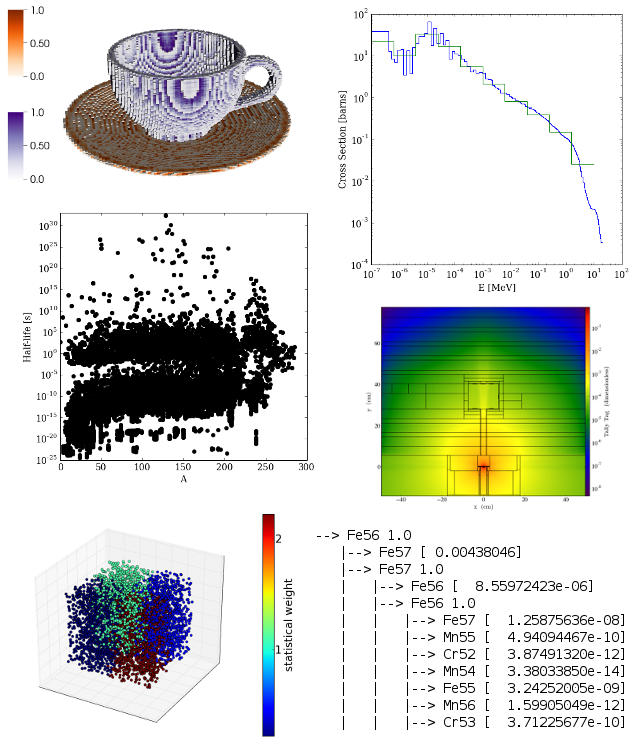
\includegraphics[width=\textwidth]{figures/pyne_splash.png}
\end{column}
\begin{column}{0.5\textwidth}
Core functionality:
\begin{itemize}
\item{Nuclide/reaction naming}
\item{Material handling}
\item{Mesh generation and operation}
\item{Cross section interface}
\item{Physics code support (MCNP5, Serpent, ALARA, ORIGEN 2.2)}
\item{Nuclear data (ACE, ENDF, ENSDF, CCCC, NJOY)}
\end{itemize}
\end{column}
\end{columns}

\end{frame}
%%%%%%%%%%%%%%%%%%%%%%%%%%%%%%%%%%%%%%%%%%%%%%%%%%%%%%%%%%%%%%%%%%%%%%%%%%%%%%%%
\begin{frame}
\frametitle{My work within PyNE}

\begin{columns}
\begin{column}{0.4\textwidth}
Mesh-based shutdown dose rate estimation for fusion energy systems \cite{Biondo2014} and corresponding hybrid MC variance reduction.
\begin{itemize}
\item{\texttt{mcnp}}
\item{\texttt{mesh}}
\item{\texttt{material} }
\item{\texttt{alara}}
\item{\texttt{dagmc}}
\item{\texttt{source sampling}}
\item{\texttt{variance reduction}}
\item{\texttt{r2s}}
\end{itemize}
\end{column}
\begin{column}{0.6\textwidth}
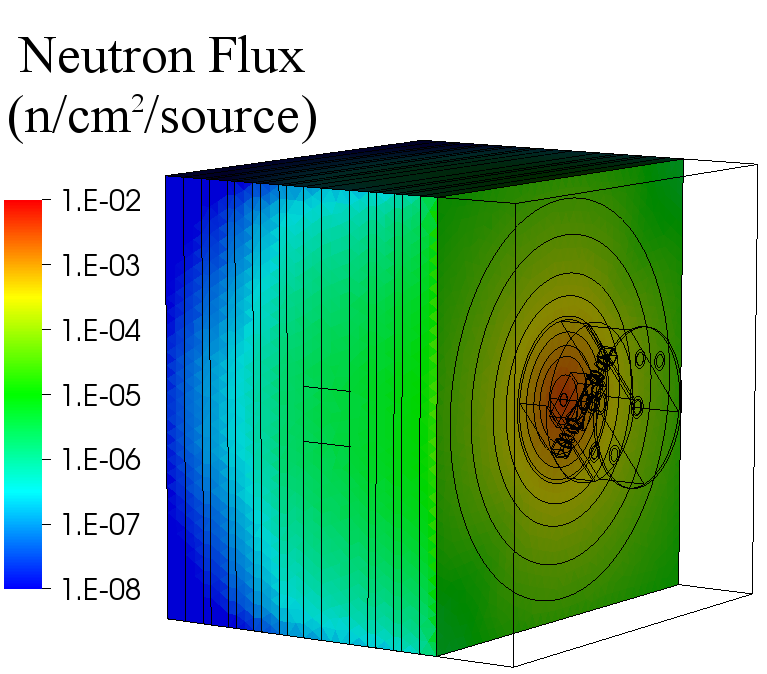
\includegraphics[width=3.8cm]{figures/n_flux.png}
\vspace{0.2cm}
{ \arrowdown} {\small Activation} \\
\centerline{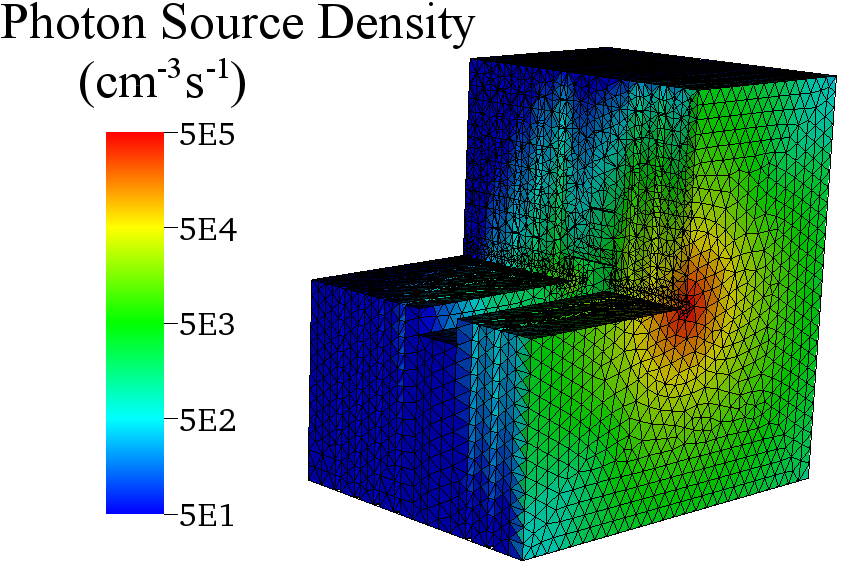
\includegraphics[width=4.2cm]{figures/phtn_src.png}}
\centerline{\hspace{0.5cm} \arrowdown {\small Photon Transport}} 
\vspace{0.2cm}
\framebox[1.1\width]{Shutdown Dose Rate}
\end{column}
\end{columns}
\end{frame}
%%%%%%%%%%%%%%%%%%%%%%%%%%%%%%%%%%%%%%%%%%%%%%%%%%%%%%%%%%%%%%%%%%%%%%%%%%%%%%%%
\begin{frame}[fragile]
\frametitle{Quality assurance}

\begin{itemize}
\item{PyNE developers have an interest in ensuring code is correct, robust,
well-documented, and easy to use}
\item{Some activities within national labs and industry require code that is compliant with NRC regulatory standards}
\item{It is worth understanding/compling with NRC regulatory standards:}
\begin{itemize}
\item{Increase potential user-base}
\item{Better product}
\end{itemize}
\end{itemize}

\end{frame}
%%%%%%%%%%%%%%%%%%%%%%%%%%%%%%%%%%%%%%%%%%%%%%%%%%%%%%%%%%%%%%%%%%%%%%%%%%%%%%%%
\begin{frame}[fragile]
\frametitle{Quality assurance in nuclear engineering}

\begin{columns}[T]
\begin{column}{0.5\textwidth}

\includegraphics[width=\textwidth]{figures/nqa-1-2008.png}
\end{column}
\begin{column}{0.5\textwidth}
\begin{itemize}
\item{American Society of Mechanical Engineers (ASME)
NQA-1-2008 \cite{nqa} standard and NQA-1a-2009 \cite{add} addendum}
\item{Endorsed by the NRC for design and construction of power plants and reprocessing facilities}
\end{itemize}
\end{column}
\end{columns}


\end{frame}
%%%%%%%%%%%%%%%%%%%%%%%%%%%%%%%%%%%%%%%%%%%%%%%%%%%%%%%%%%%%%%%%%%%%%%%%%%%%%%%%
\begin{frame}[fragile]
\frametitle{Objective}

\begin{enumerate}
\item{What software development practices are prescribed by NQA-1?}
\item{How do PyNE's practices map to the criteria set forth in NQA-1?}
\end{enumerate}

\end{frame}

%%%%%%%%%%%%%%%%%%%%%%%%%%%%%%%%%%%%%%%%%%%%%%%%%%%%%%%%%%%%%%%%%%%%%%%%%%%%%%%%
%%%%%%%%%%%%%%%%%%%%%%%%%%%%%%%%%%%%%%%%%%%%%%%%%%%%%%%%%%%%%%%%%%%%%%%%%%%%%%%%
%%%%%%%%%%%%%%%%%%%%%%%%%%%%%%%%%%%%%%%%%%%%%%%%%%%%%%%%%%%%%%%%%%%%%%%%%%%%%%%%
\section{NQA-1 standard}
%%%%%%%%%%%%%%%%%%%%%%%%%%%%%%%%%%%%%%%%%%%%%%%%%%%%%%%%%%%%%%%%%%%%%%%%%%%%%%%%
%%%%%%%%%%%%%%%%%%%%%%%%%%%%%%%%%%%%%%%%%%%%%%%%%%%%%%%%%%%%%%%%%%%%%%%%%%%%%%%%
%%%%%%%%%%%%%%%%%%%%%%%%%%%%%%%%%%%%%%%%%%%%%%%%%%%%%%%%%%%%%%%%%%%%%%%%%%%%%%%%

\begin{frame}[fragile]
\frametitle{The Waterfall method}
\centerline{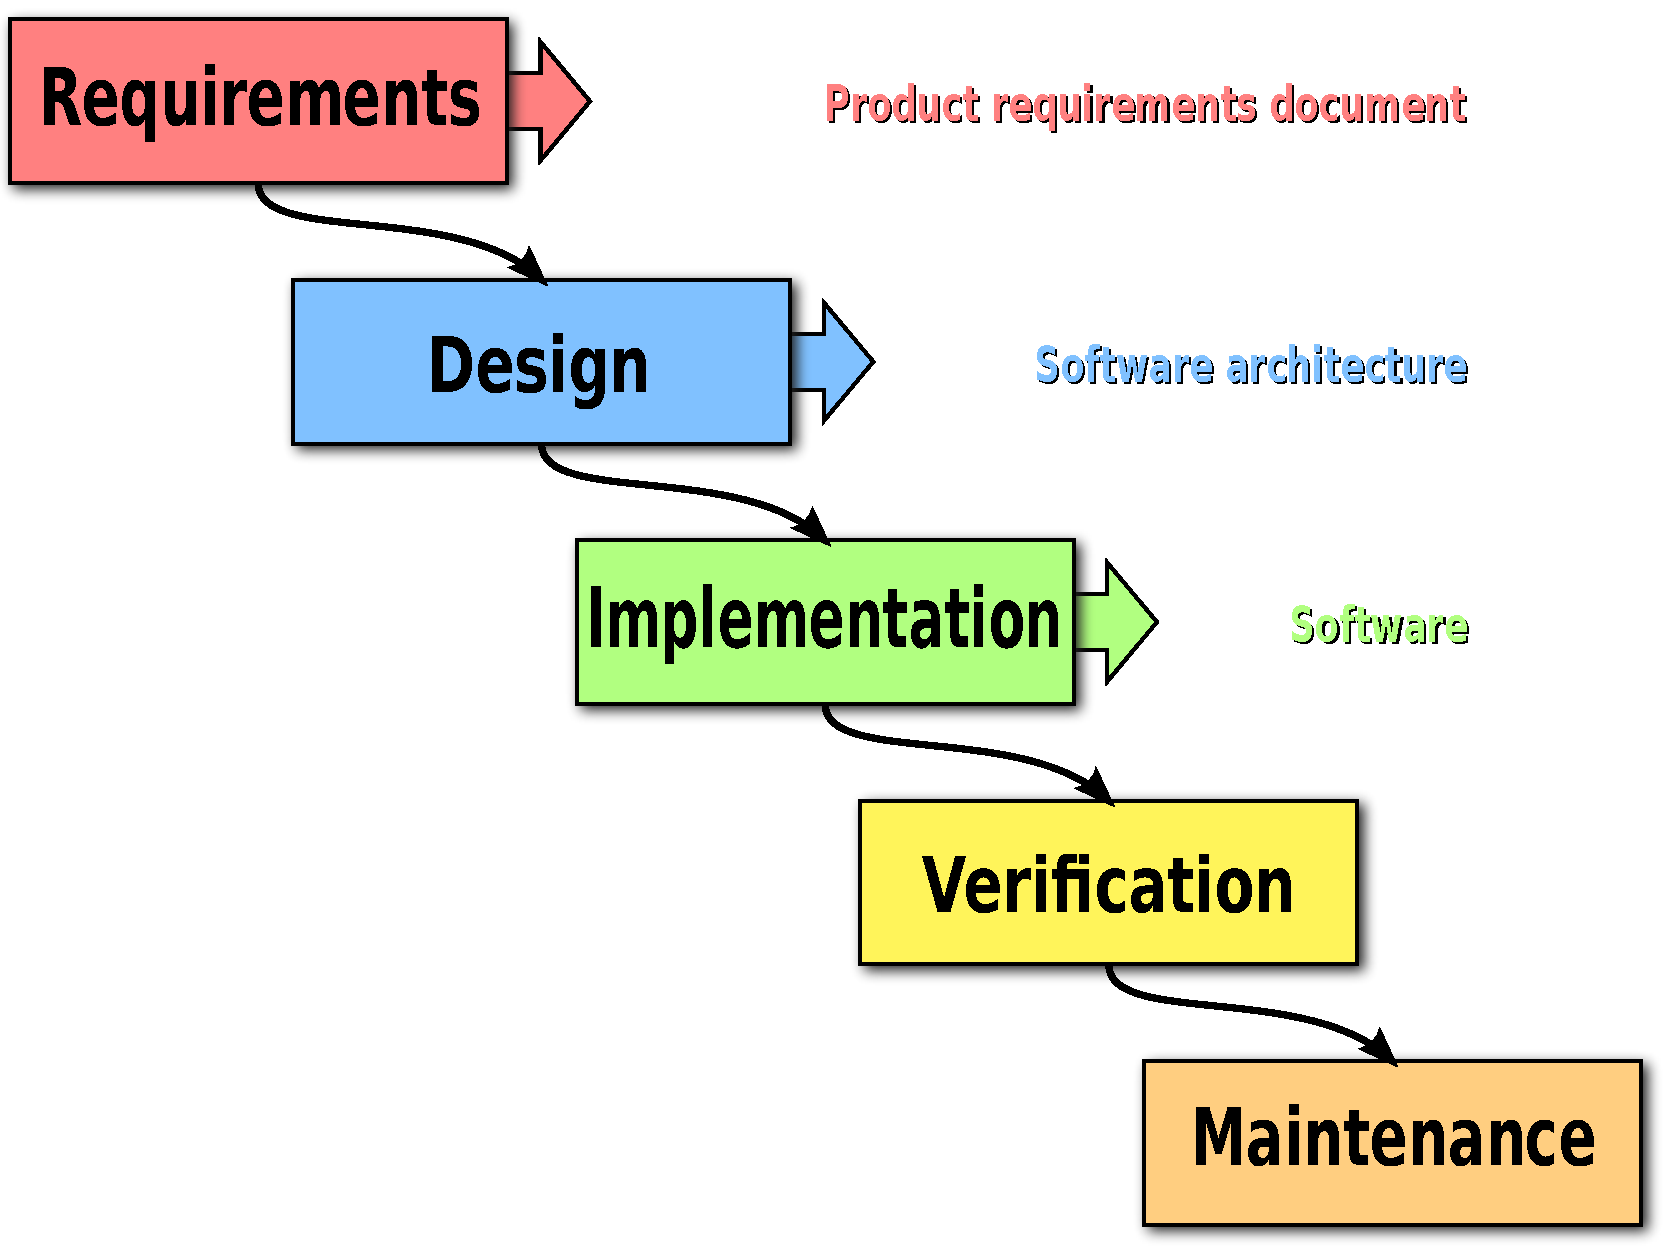
\includegraphics[width=0.8\textwidth]{figures/waterfall.pdf}}
Waterfall method \cite{waterfall}, figure from \cite{waterfall_wiki}
\end{frame}

%%%%%%%%%%%%%%%%%%%%%%%%%%%%%%%%%%%%%%%%%%%%%%%%%%%%%%%%%%%%%%%%%%%%%%%%%%%%%%%%
\begin{frame}
\frametitle{NQA-1 Part I}

{\bf Part I: ``Requirements for Quality Assurance Programs for Nuclear Facilities''}

Requirement 3 Section 801:
\begin{enumerate}
\item{\alert{Requirements} - the scope of the capabilities implemented by the work}
\item{\alert{Software design} - the mathematical and computational methodologies employed to meet the requirements}
\item{\alert{Implementation} - writing code using the standards and conventions agreed upon by the organization}
\item{\alert{Software design verification} - independent confirmation that requirements are met}
\item{\alert{Computer program testing} - comparison of results produced by the work to expected or known results}
\end{enumerate}
\end{frame}

%%%%%%%%%%%%%%%%%%%%%%%%%%%%%%%%%%%%%%%%%%%%%%%%%%%%%%%%%%%%%%%%%%%%%%%%%%%%%%%%
\begin{frame}
\frametitle{NQA-1 Part I (cont.)}

Requirement 2 Section 802:
\begin{itemize}
\item{\alert{Configuration identification} - identify each version of the code and the difference between them}
\item{\alert{Configuration change control} - document changes to the baseline as well as justification/verification}
\item{\alert{Configuration status control} - accounted for prior to being incorporated into the baseline and changes that are “proposed and approved, but not implemented” are documented \cite{add}}
\end{itemize}
\end{frame}
%%%%%%%%%%%%%%%%%%%%%%%%%%%%%%%%%%%%%%%%%%%%%%%%%%%%%%%%%%%%%%%%%%%%%%%%%%%%%%%%
\begin{frame}
\frametitle{Part II}

{\bf Part II: ``Quality Assurance Requirements for Facility Applications''}

\begin{itemize}
\item{Section 301: \alert{Otherwise Acquired software} - Additional QA is required for software dependencies ``not previously approved under a program consistent with this standard''}
\item{Section 204: \alert{Problem reporting} and \alert{corrective action}}
\item{Section 500: \alert{Standards}, \alert{conventions}, and other \alert{work practices}}
\end{itemize}

%Only relevant to end user applications:
%\begin{itemize}
%\item{Section 401-404 - Security Requirements}
%\item{Section 405 - Operation Requirements}
%\item{Section 600 - Software Tools and System Software}
%\end{itemize}
\end{frame}
%%%%%%%%%%%%%%%%%%%%%%%%%%%%%%%%%%%%%%%%%%%%%%%%%%%%%%%%%%%%%%%%%%%%%%%%%%%%%%%%%
\begin{frame}
\frametitle{Applicability of NQA-1}

\alert{Otherwise acquired software} section - provisions for the use of
``freeware'' that ``has not been previously approved under a program consistent
with [the NQA-1 standard]''

\begin{itemize}
\item{PyNE as an organization will never need official NQA-1 compliance}
    \begin{itemize}
    \item{Unless we decide to build a power plant!}
    \end{itemize}
\item{It is more likely PyNE code may be a component within an end-user application used for activities requiring compliance}
\item{It is worth being consistent with this standard, so this Subpart could be evoked}
    \begin{itemize}
    \item{QA burden for third parties is lessened}
    \end{itemize}
\end{itemize}

\end{frame}

%%%%%%%%%%%%%%%%%%%%%%%%%%%%%%%%%%%%%%%%%%%%%%%%%%%%%%%%%%%%%%%%%%%%%%%%%%%%%%%%%
%%%%%%%%%%%%%%%%%%%%%%%%%%%%%%%%%%%%%%%%%%%%%%%%%%%%%%%%%%%%%%%%%%%%%%%%%%%%%%%%%
%%%%%%%%%%%%%%%%%%%%%%%%%%%%%%%%%%%%%%%%%%%%%%%%%%%%%%%%%%%%%%%%%%%%%%%%%%%%%%%%%
\section{QA within PyNE}
%%%%%%%%%%%%%%%%%%%%%%%%%%%%%%%%%%%%%%%%%%%%%%%%%%%%%%%%%%%%%%%%%%%%%%%%%%%%%%%%%
%%%%%%%%%%%%%%%%%%%%%%%%%%%%%%%%%%%%%%%%%%%%%%%%%%%%%%%%%%%%%%%%%%%%%%%%%%%%%%%%%
%%%%%%%%%%%%%%%%%%%%%%%%%%%%%%%%%%%%%%%%%%%%%%%%%%%%%%%%%%%%%%%%%%%%%%%%%%%%%%%%%
%
%%%%%%%%%%%%%%%%%%%%%%%%%%%%%%%%%%%%%%%%%%%%%%%%%%%%%%%%%%%%%%%%%%%%%%%%%%%%%%%%%
%\begin{frame}
%\frametitle{Forewarning}
%
%\begin{itemize}
%\item{This is a developer's perspective.}
%\item{Knowledge of the activities discussed here not prerequisite for users.}
%\end{itemize}
%
%\end{frame}
%

%%%%%%%%%%%%%%%%%%%%%%%%%%%%%%%%%%%%%%%%%%%%%%%%%%%%%%%%%%%%%%%%%%%%%%%%%%%%%%%%
\begin{frame}[fragile]
\frametitle{Challenges}

\begin{itemize}
\item{PyNE code is heterogeneous:}
    \begin{itemize}
    \item{Research vs.\ production level}
    \item{``Library'' code vs.\ end-user applications}
    \item{Some modules involve physics, others do not}
    \end{itemize}
\item{PyNE developers are a diverse bunch}:
   \begin{itemize}
   \item{Experience: Undergraduates through professors}
   \item{Ability: Varying levels of software development background}
   \item{Effort: Spare time vs.\ funded work}
   \end{itemize}
\end{itemize}

\end{frame}
%%%%%%%%%%%%%%%%%%%%%%%%%%%%%%%%%%%%%%%%%%%%%%%%%%%%%%%%%%%%%%%%%%%%%%%%%%%%%%%%
\begin{frame}
\frametitle{Agile software development}

Agile Software Development \cite{larman2004agile}:
\begin{itemize}
\item{All developers access a reliable software baseline, make changes, and request that the changes become the new baseline}
\item{Each change is analogous to a mini-waterfall method}
\end{itemize}

\centerline{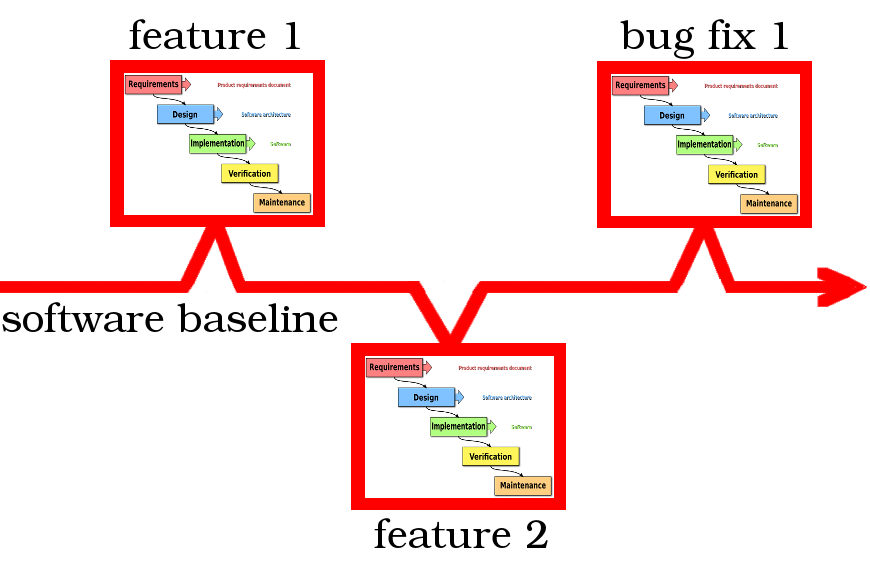
\includegraphics[width=0.8\textwidth]{figures/agile.png}}

\end{frame}
%%%%%%%%%%%%%%%%%%%%%%%%%%%%%%%%%%%%%%%%%%%%%%%%%%%%%%%%%%%%%%%%%%%%%%%%%%%%%%%%
\begin{frame}
\frametitle{Agile software development}

\begin{itemize}
\item{Better for projects that are:}
    \begin{itemize}
    \item{Decentralized}
    \item{On-going}
    \end{itemize}
\item{Made possible by:}
    \begin{itemize}
    \item{Version control}
    \item{Unit tests}
    \item{Continuous integration}
    \end{itemize}
\end{itemize}

\end{frame}


%%%%%%%%%%%%%%%%%%%%%%%%%%%%%%%%%%%%%%%%%%%%%%%%%%%%%%%%%%%%%%%%%%%%%%%%%%%%%%%%
\begin{frame}
\frametitle{Version control}

All code, tests, and documentation are version controlled using Git \cite{git} \\
\vspace{0.3cm}
Git (like Mercurial, SVN, or CVS) is software that allows users to:
\begin{itemize}
\item{Assign a unique identifier to a version of a code base, e.g., a snapshot of 
      the code after a developer makes changes (\alert{configuration identification})}
\item{Compare, merge, or revert to different versions}
\item{Permanently store all versions of code in a \emph{repository} (\alert{configuration change control})}
\end{itemize}
\vspace{0.3cm}
The PyNE Git repository is hosted on GitHub.com

\end{frame}

%%%%%%%%%%%%%%%%%%%%%%%%%%%%%%%%%%%%%%%%%%%%%%%%%%%%%%%%%%%%%%%%%%%%%%%%%%%%%%%%
\begin{frame}
\frametitle{Pull requests}

\begin{columns}
\begin{column}{0.5\textwidth}

Developers
    \begin{itemize}
    \item Create their own copy of the repository -- a``fork'' (\alert{configuration status control})
    \item Make changes
    \item Request that the changes get applied the baseline
    \end{itemize}
\end{column}
\begin{column}{0.5\textwidth}
    \centerline{example:}
    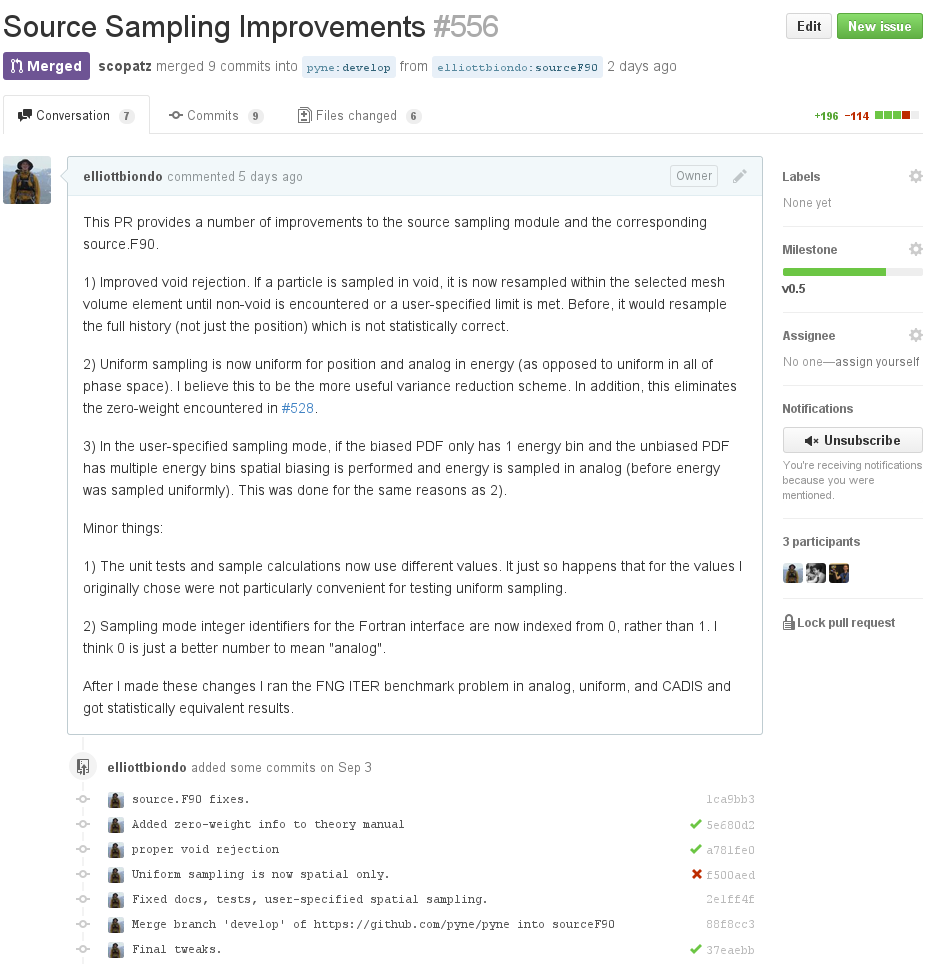
\includegraphics[width=\textwidth]{figures/PR_prop.png}
\end{column}
\end{columns}

\end{frame}

%%%%%%%%%%%%%%%%%%%%%%%%%%%%%%%%%%%%%%%%%%%%%%%%%%%%%%%%%%%%%%%%%%%%%%%%%%%%%%%%
\begin{frame}
\frametitle{Pull requests}

\begin{columns}
\begin{column}{0.5\textwidth}

Other developers/reviewers
    \begin{itemize}
    \item{Review by someone who did not write the code (\alert{software design verification})}
    \visible<2->{\item{Iterative process}}
    \visible<3->{\item{Permanently saved (\alert{configuration change control})}}
    \end{itemize}
\end{column}
\begin{column}{0.5\textwidth}
    \only<1>{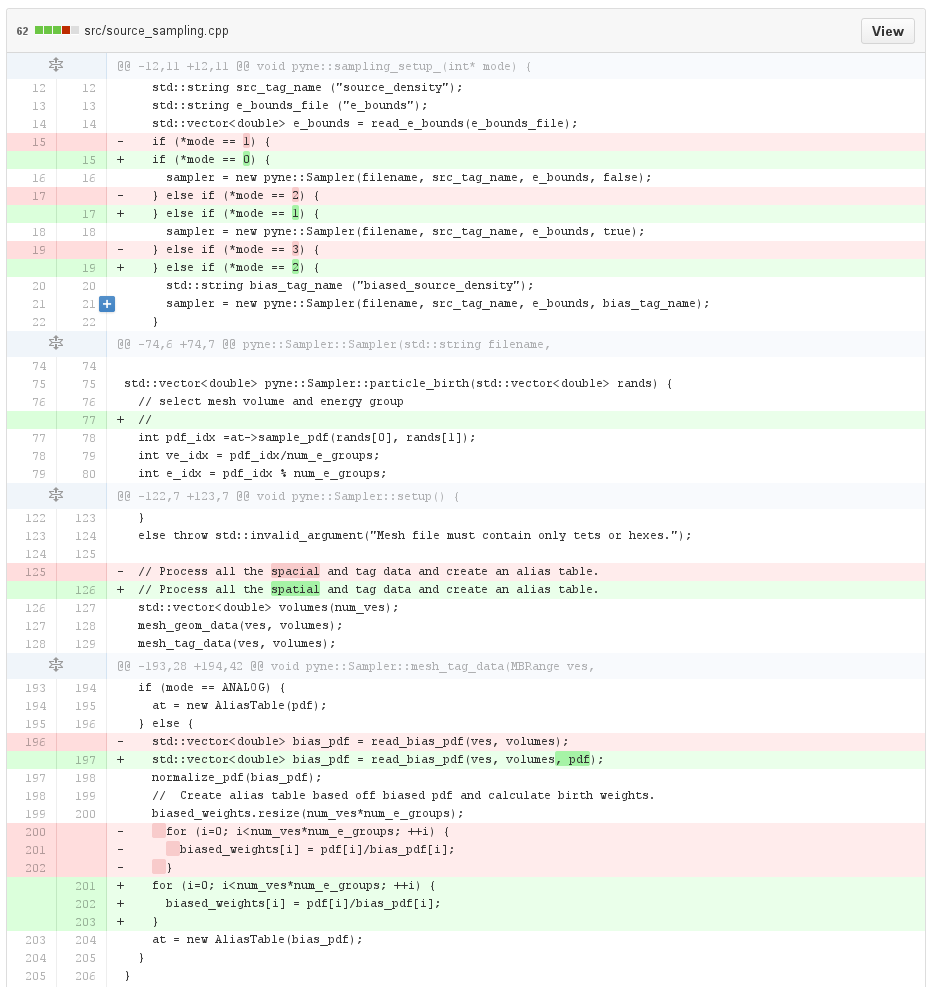
\includegraphics[width=\textwidth]{figures/PR_review.png}}
    \only<2>{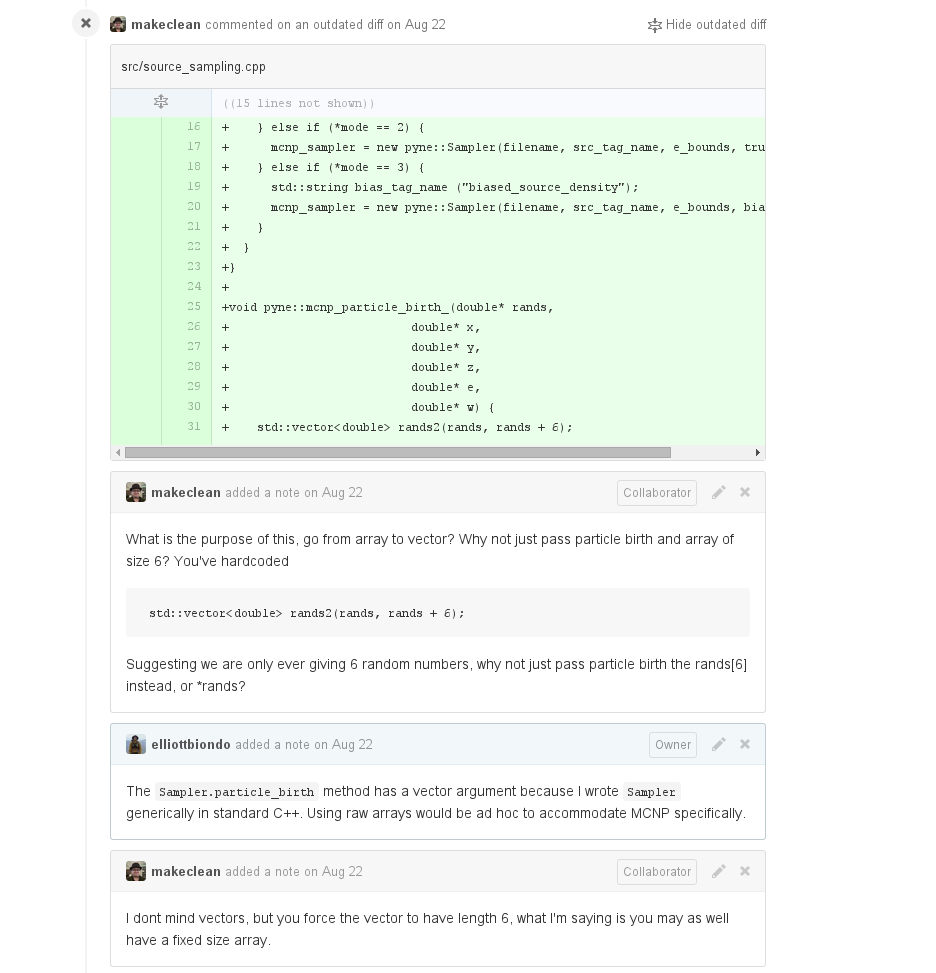
\includegraphics[width=\textwidth]{figures/PR_iterative.png}}
    \only<3>{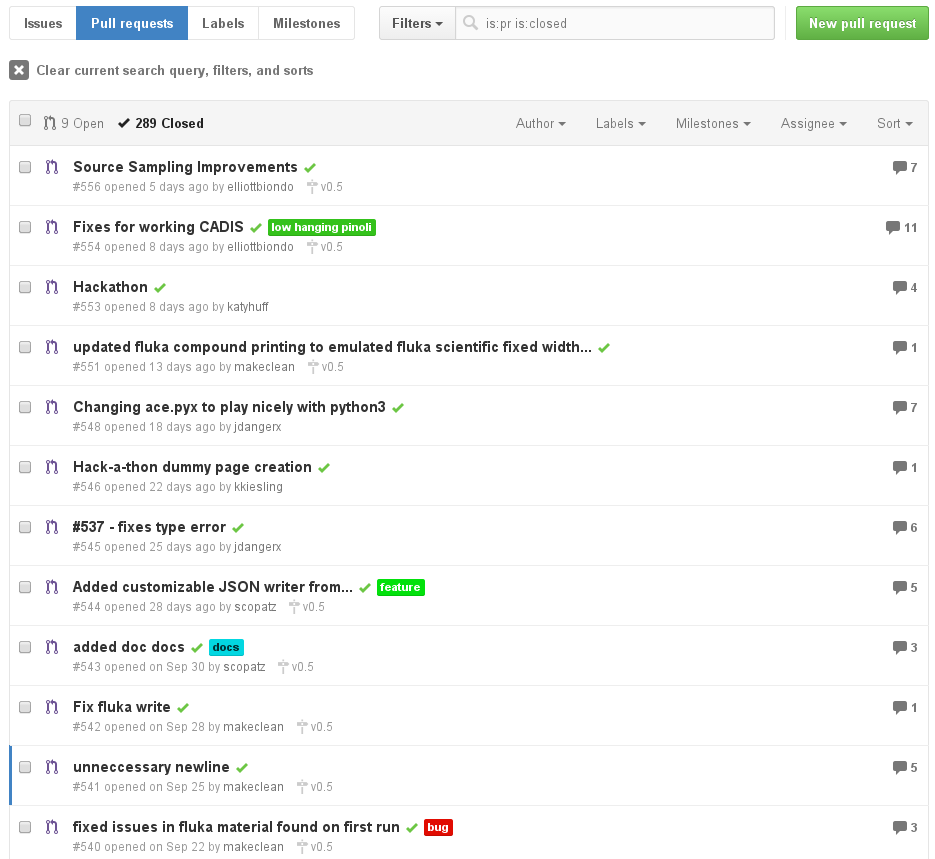
\includegraphics[width=\textwidth]{figures/PR_closed.png}}
\end{column}
\end{columns}

\end{frame}

%%%%%%%%%%%%%%%%%%%%%%%%%%%%%%%%%%%%%%%%%%%%%%%%%%%%%%%%%%%%%%%%%%%%%%%%%%%%%%%%
\begin{frame}
\frametitle{Requirements for pull requests}

In order to be accepted:

\begin{itemize}
\item{Explanation and justification for the changes (\alert{requirements})}
\item{Unit tests that cover any new features (\alert{computer program testing})}
\item{All pre-existing unit tests pass}
\item{Inline documentation}
\item{Format compliant with the PyNE Style guide (\alert{implementation})}
\end{itemize}

\end{frame}

%%%%%%%%%%%%%%%%%%%%%%%%%%%%%%%%%%%%%%%%%%%%%%%%%%%%%%%%%%%%%%%%%%%%%%%%%%%%%%%%
\begin{frame}
\frametitle{Continuous integration}

Continuous Integration \cite{beck1998extreme}:

\begin{itemize}
\item{Upon receiving a pull request, a developer's code is built and tested on a remote server}
    \begin{itemize}
    \item{4 \emph{platforms}:}
        \begin{itemize}
        \item{Ubuntu 12}
        \item{Mac OSX8}
        \item{Scientific Linux 6}
        \item{Ubuntu 10 with Python 3}
        \end{itemize}
    \end{itemize}
\item{UW Build and Test Lab (BaTLab) \cite{batlab_2014}}
\item{Integrated with GitHub using Polyphemus \cite{polyphemus_2014}}
\end{itemize}
\end{frame}

%%%%%%%%%%%%%%%%%%%%%%%%%%%%%%%%%%%%%%%%%%%%%%%%%%%%%%%%%%%%%%%%%%%%%%%%%%%%%%%%
\begin{frame}
\frametitle{Continuous integration}

The view from GitHub:
\only<1>{\centerline{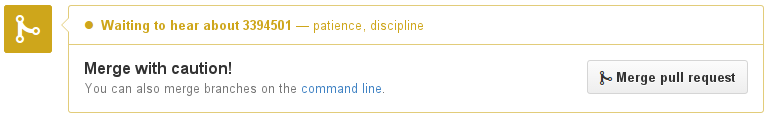
\includegraphics[width=\textwidth]{figures/CI_wait.png}}}
\only<2>{\centerline{
\includegraphics[width=\textwidth]{figures/CI_pass.png}}}
\only<3>{\centerline{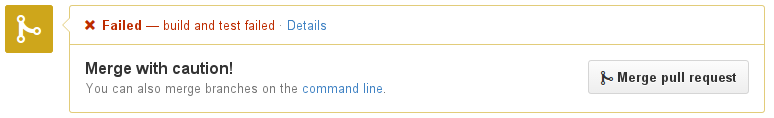
\includegraphics[width=\textwidth]{figures/CI_fail.png}}\vspace{0.5cm}}

When a pull request is initiated, BaTLab automatically:
\begin{enumerate}
\visible<1->{
\item{Installs PyNE's dependencies}
\item{Builds and installs PyNE with the developer's changes}
\item{Runs all unit tests}
}
\visible<2->{
\item{Reports results}
}
\end{enumerate}

\end{frame}
%%%%%%%%%%%%%%%%%%%%%%%%%%%%%%%%%%%%%%%%%%%%%%%%%%%%%%%%%%%%%%%%%%%%%%%%%%%%%%%%
\begin{frame}
\frametitle{Continuous integration}

Detailed output:
\centerline{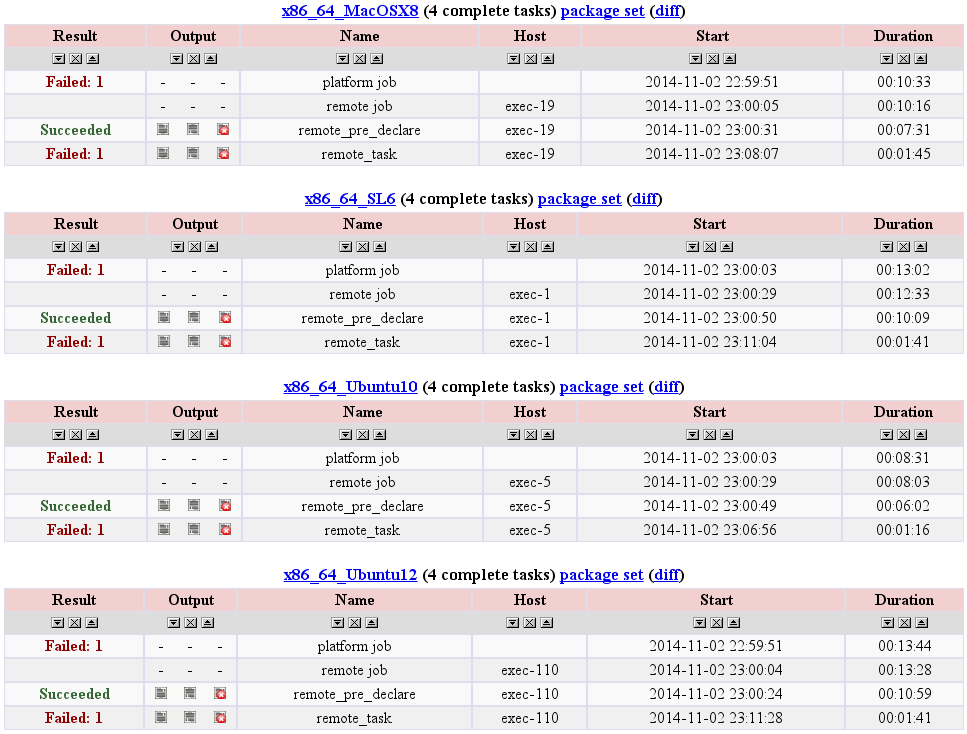
\includegraphics[height=0.8\textheight]{figures/CI_detail.png}}

\end{frame}
%%%%%%%%%%%%%%%%%%%%%%%%%%%%%%%%%%%%%%%%%%%%%%%%%%%%%%%%%%%%%%%%%%%%%%%%%%%%%%%%
\begin{frame}
\frametitle{Nightly testing}

\begin{itemize}
\item{Same procedure as CI, but occurs every 24 hours}
\item{PyNE mailing list is notified in the case of any failures}
\item{Will come in handy when long regression tests are added}
\end{itemize}


\end{frame}

%%%%%%%%%%%%%%%%%%%%%%%%%%%%%%%%%%%%%%%%%%%%%%%%%%%%%%%%%%%%%%%%%%%%%%%%%%%%%%%%
\begin{frame}
\frametitle{Infrastructure}

\begin{columns}
\begin{column}{0.5\textwidth}
    \begin{itemize}
    \item{Website: \url{pyne.io}}
    \begin{itemize}
    \visible<2->{\item{Developer's guide} (\alert{standards}, \alert{conventions}, \alert{work practices})}
    \visible<3->{\item{User's guide}}
    \visible<4->{\item{Theory manual - still under development}}
    \end{itemize}
    \visible<5->{
    \item{User mailing list (\alert{problem reporting})}
    \item{Developer mailing list}
    }
    \end{itemize}
\end{column}
\begin{column}{0.5\textwidth}
    \only<1>{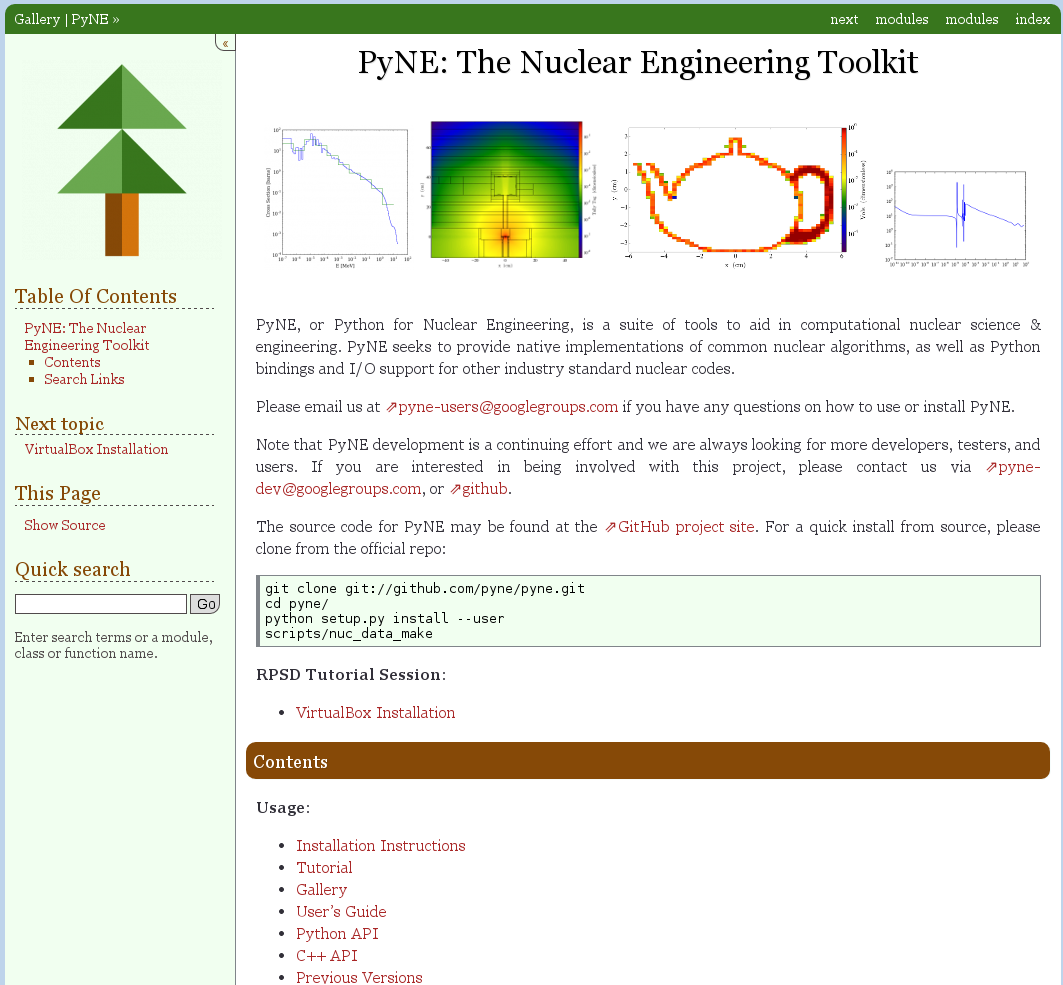
\includegraphics[width=\textwidth]{figures/inf_website.png}}
    \only<2>{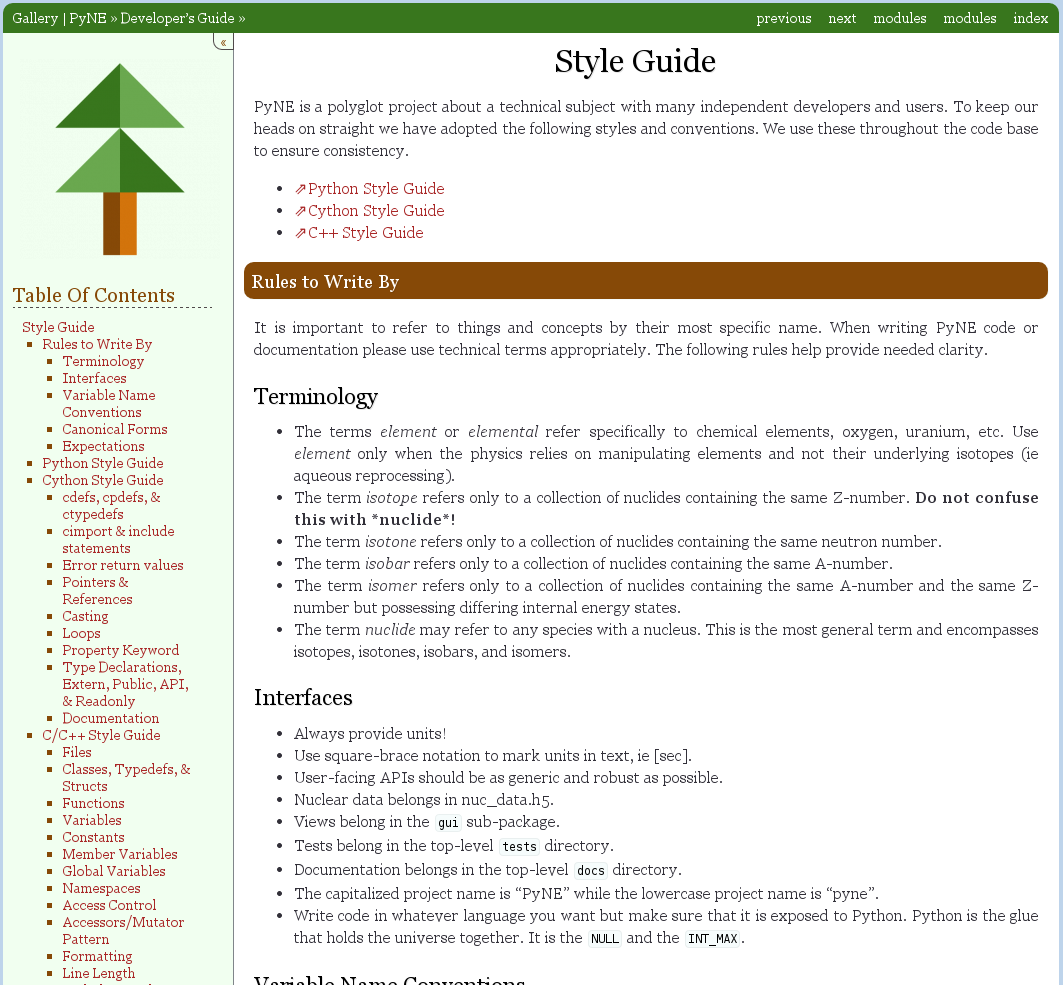
\includegraphics[width=\textwidth]{figures/inf_dev.png}}
    \only<3>{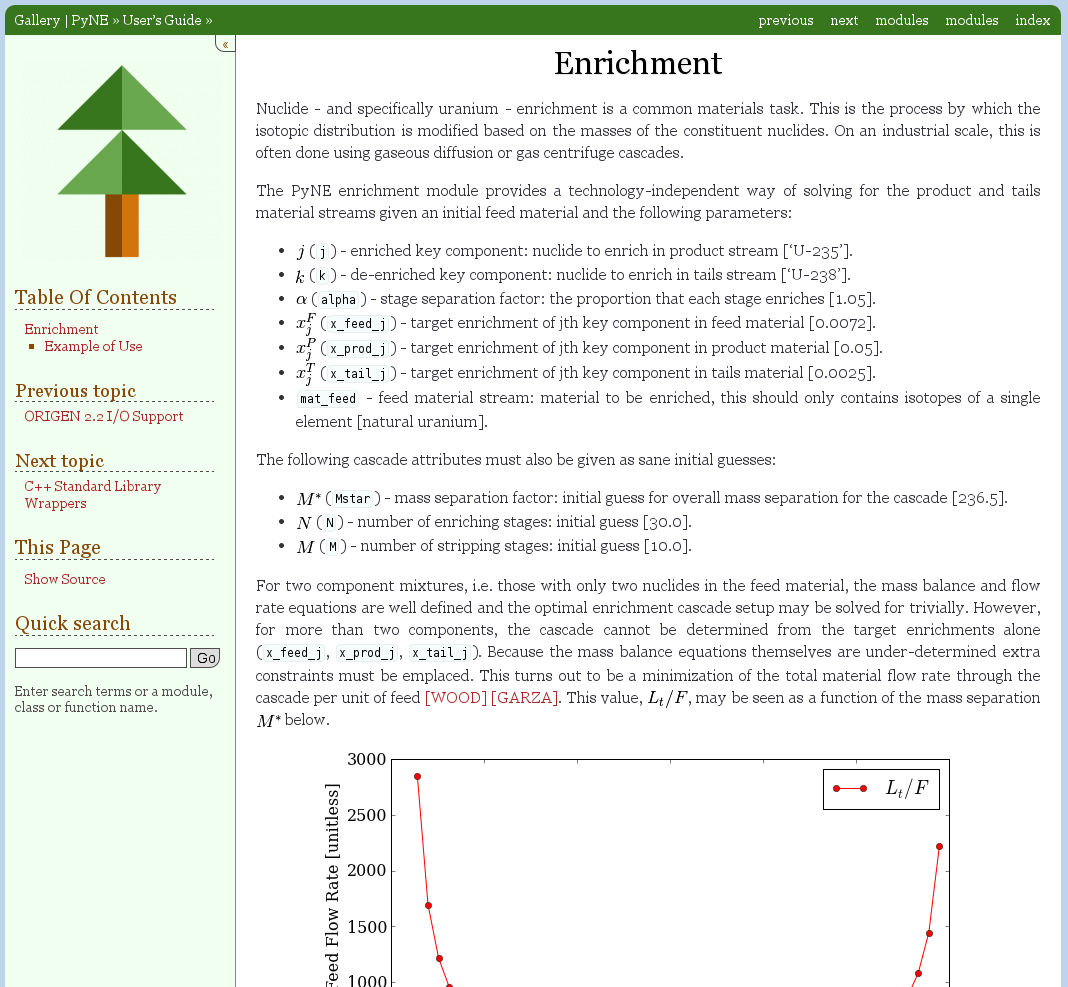
\includegraphics[width=\textwidth]{figures/inf_user.png}}
    \only<4>{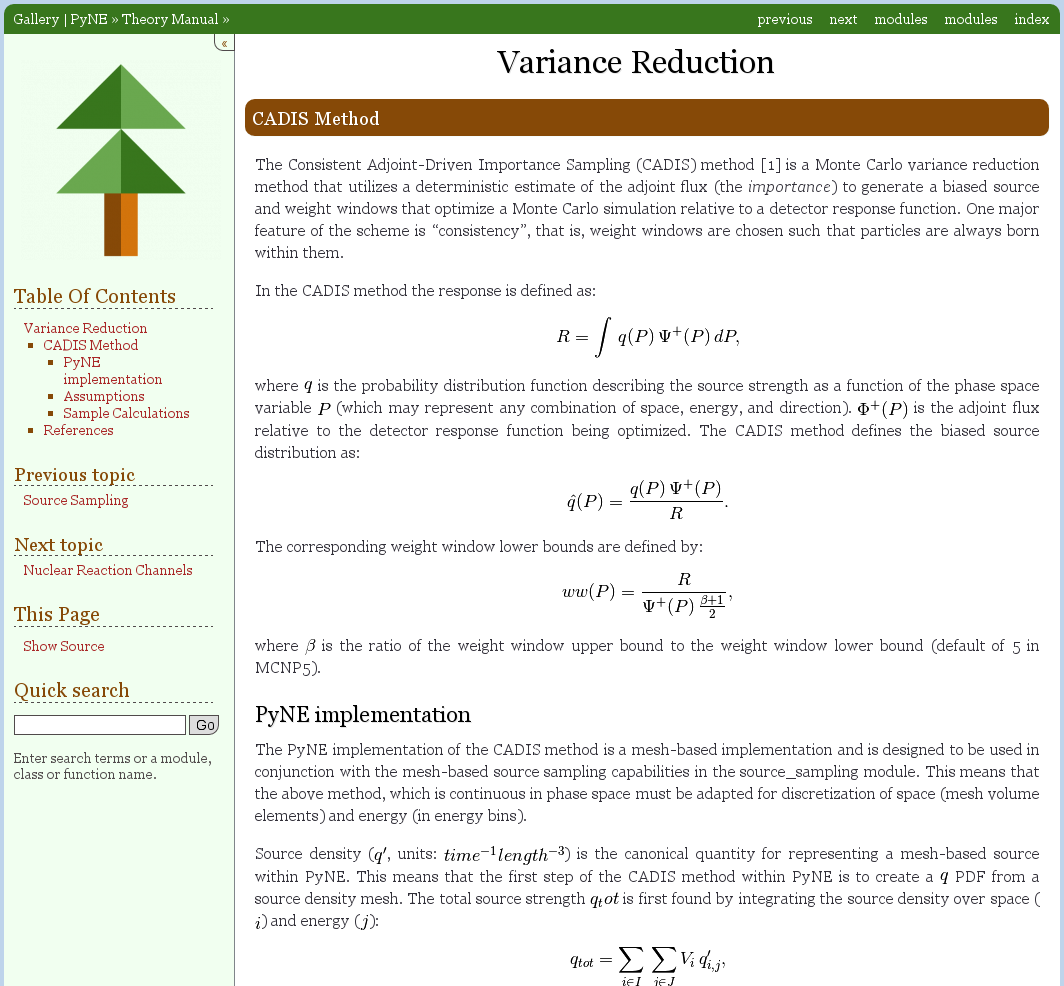
\includegraphics[width=\textwidth]{figures/inf_theory.png}}
    \only<5>{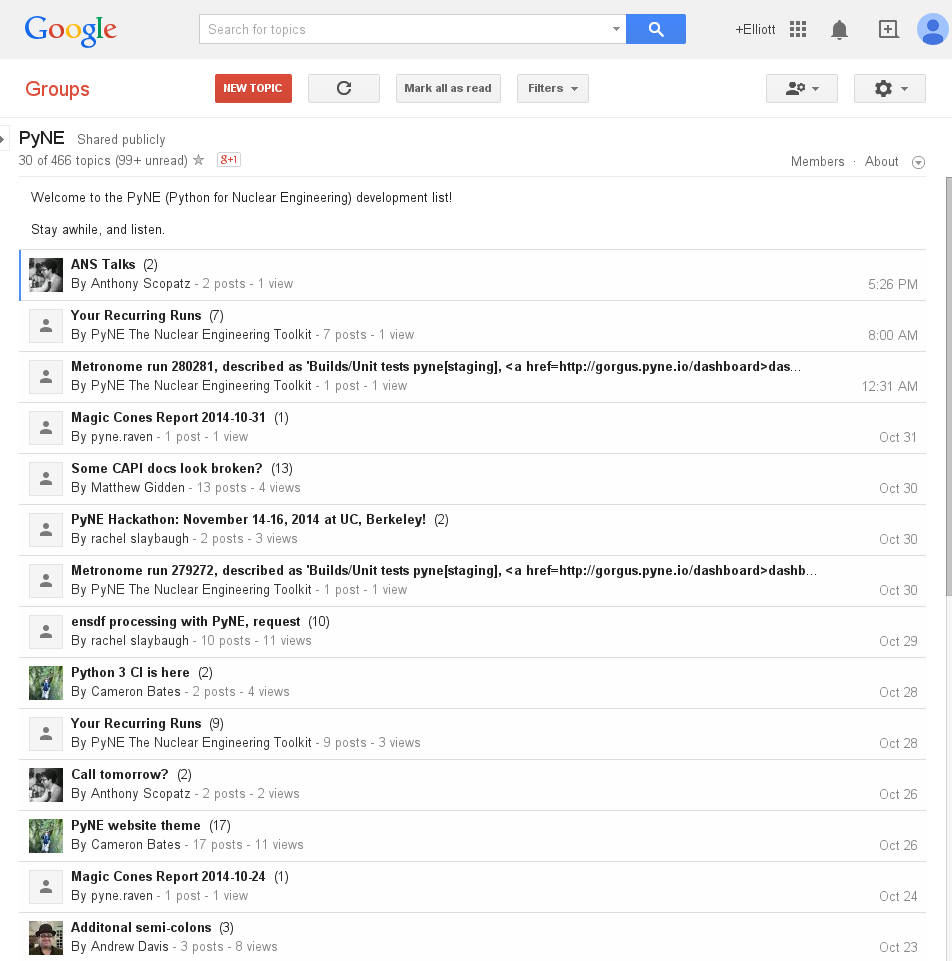
\includegraphics[width=\textwidth]{figures/inf_mail.png}}
\end{column}
\end{columns}

\end{frame}


%%%%%%%%%%%%%%%%%%%%%%%%%%%%%%%%%%%%%%%%%%%%%%%%%%%%%%%%%%%%%%%%%%%%%%%%%%%%%%%%
\begin{frame}
\frametitle{The PyNE QA standard}

\begin{itemize}
\item{Almost everything heretofore has been the bare minimum to be accepted into PyNE}
\item{What does it take for code within PyNE to be declared ``QA complaint''?}
    \begin{itemize}
    \item{Fill in gaps between pull request criteria and NQA-1 criteria}
    \end{itemize}
\end{itemize}

\end{frame}

%%%%%%%%%%%%%%%%%%%%%%%%%%%%%%%%%%%%%%%%%%%%%%%%%%%%%%%%%%%%%%%%%%%%%%%%%%%%%%%%
\begin{frame}
\frametitle{The PyNE QA standard}

Declaring modules QA compliant:
\begin{enumerate}
\item{Theory manual entry}:
    \begin{itemize}
    \item{Explains/cites all mathematics/physics that occur}
    \item{Assumptions/limitations}
    \item{Sample calculations for numbers that appear in unit tests}
    \end{itemize}
\item{Unit test coverage spans the entire set of capabilities described in the theory manual}
\item{User manual entry that describes how to use a given module}
\item{For modules with significant physics (e.g.\ transport, transmutation):}
    \begin{itemize}
    \item{benchmarking experimental results}
    \item{appropriate uncertainty and sensitivity analysis}
    \item{regression tests must be incorporated into the CI}
    \end{itemize}
\end{enumerate}

\end{frame}

%%%%%%%%%%%%%%%%%%%%%%%%%%%%%%%%%%%%%%%%%%%%%%%%%%%%%%%%%%%%%%%%%%%%%%%%%%%%%%%%
\begin{frame}
\frametitle{Work to date}

\begin{itemize}
\item{Ratified QA plan}
\item{One module fully compliant (\texttt{pyne.nucname})}
\item{Major topic at the PyNE 3-day Hack-a-thon at UC-Berkeley this weekend}
\end{itemize}

\end{frame}
%%%%%%%%%%%%%%%%%%%%%%%%%%%%%%%%%%%%%%%%%%%%%%%%%%%%%%%%%%%%%%%%%%%%%%%%%%%%%%%%
\begin{frame}
\frametitle{Conclusion}

\begin{itemize}
\item{The software development practices within PyNE accomplish the same goals as NQA-1}
\item{In the future, if some party were to use a QA-compliant portion of PyNE for NQA-1 compliant code, much of the QA work will already be done}
\end{itemize}

\end{frame}
%%%%%%%%%%%%%%%%%%%%%%%%%%%%%%%%%%%%%%%%%%%%%%%%%%%%%%%%%%%%%%%%%%%%%%%%%%%%%%%%
\begin{frame}[fragile]
\frametitle{Acknowledgments}


\includegraphics[height=2cm]{figures/NRClogo.png} \\

\end{frame}

%%%%%%%%%%%%%%%%%%

%%%%%%%%%%%%%%%%%%%%%%%%%%%%%%%%%%%%%%%%%%%%%%%%%%%%%%%%%%%%%%%%%%%%%%%%%%%%%%%%
%%%%%%%%%%%%%%%%%%%%%%%%%%%%%%%%%%%%%%%%%%%%%%%%%%%%%%%%%%%%%%%%%%%%%%%%%%%%%%%%
%%%%%%%%%%%%%%%%%%%%%%%%%%%%%%%%%%%%%%%%%%%%%%%%%%%%%%%%%%%%%%%%%%%%%%%%%%%%%%%%
\section*{Questions?}
%%%%%%%%%%%%%%%%%%%%%%%%%%%%%%%%%%%%%%%%%%%%%%%%%%%%%%%%%%%%%%%%%%%%%%%%%%%%%%%%
%%%%%%%%%%%%%%%%%%%%%%%%%%%%%%%%%%%%%%%%%%%%%%%%%%%%%%%%%%%%%%%%%%%%%%%%%%%%%%%%
%%%%%%%%%%%%%%%%%%%%%%%%%%%%%%%%%%%%%%%%%%%%%%%%%%%%%%%%%%%%%%%%%%%%%%%%%%%%%%%%

%\begin{frame}[allowframebreaks]
\begin{frame}[plain]
        \tiny
        \frametitle{References}
        \bibliographystyle{ans}
        \color{black}
        \bibliography{refs}
\end{frame}

%%%%%%%%%%%%%%%%%%%%%%%%%%%%%%%%%%%%%%%%%%%%%%%%%%%%%%%%%%%%%%%%%%%%%%%%%%%%%%%%
%%%%%%%%%%%%%%%%%%%%%%%%%%%%%%%%%%%%%%%%%%%%%%%%%%%%%%%%%%%%%%%%%%%%%%%%%%%%%%%%
%%%%%%%%%%%%%%%%%%%%%%%%%%%%%%%%%%%%%%%%%%%%%%%%%%%%%%%%%%%%%%%%%%%%%%%%%%%%%%%%
\end{document}
%%%%%%%%%%%%%%%%%%%%%%%%%%%%%%%%%%%%%%%%%%%%%%%%%%%%%%%%%%%%%%%%%%%%%%%%%%%%%%%%
%%%%%%%%%%%%%%%%%%%%%%%%%%%%%%%%%%%%%%%%%%%%%%%%%%%%%%%%%%%%%%%%%%%%%%%%%%%%%%%%
